\documentclass[aps,prl,amsmath,amssymb,floatfix,notitlepage]{revtex4-1}
%\documentclass[journal=ancac3,layout=twocolumn,manuscript=article]{achemso}

\newcommand*\mycommand[1]{\texttt{\emph{#1}}}
%\newcommand*{\INTERNAL}{}
\usepackage{chemformula} % Formula subscripts using \ch{}
\usepackage[T1]{fontenc} % Use modern font encodings
\usepackage{graphicx}% Include figure files
\usepackage{dcolumn}% Align table columns on decimal point
\usepackage{bm}% bold math
\usepackage{hyperref}% add hypertext capabilities
%\hypersetup{colorlinks=true,urlcolor={blue},citecolor={blue}, linkcolor={blue}}
\usepackage{amsmath} % or simply amstext
%\newcommand{\angstrom}{\textup{\angstrom}}
\usepackage{siunitx}
\usepackage{color}
\usepackage[normalem]{ulem}
\usepackage{diagbox}
\usepackage{import}
\usepackage{multirow}
\usepackage{xr} % referencing across multiple files
\usepackage{cleveref} % cite figures in SI

%RZK: do not edit red text
\newcommand{\lock}{\color{red}}

\renewcommand{\figurename}{Supporting Figure}
\renewcommand{\tablename}{Supporting Table}
\renewcommand{\thefigure}{S\arabic{figure}}
\renewcommand{\thetable}{S\arabic{table}}

\newcommand{\sinfo}{Supporting Information}

% Use main text labels
\externaldocument[main-]{main}

\begin{document}

%RZZK: check that article titles match here and in the main text
\title{\sinfo\ for \\
Role of adatoms in the surface-confined Ullmann coupling of phenyl groups}% Force line breaks with \\
%\thanks{A footnote to the article title}%

\author{Zhenzhe Zhang}
\author{Dmitrii F. Perepichka}%
\email{dmitrii.perepichka@mcgill.ca}
\author{Rustam Z. Khaliullin}
\email{rustam.khaliullin@mcgill.ca}
\affiliation{%
 Department of Chemistry, McGill University, 801 Sherbrooke St West, Montreal, QC H3A 0B8, Canada
 %This line break forced with \textbackslash\textbackslash
}%

%\date{\today}% It is always \today, today,
             %  but any date may be explicitly specified

\maketitle

%The mechanism of classical Ullmann coupling is relatively well understood (Fig.~\ref{fig:classical}).
%%The Ullmann coupling reactions discussed above occur mostly in organic solvents. 
%It is widely accepted that an aryl halides molecule reacts with Cu species to form an organometallic intermediate. 
%This intermediate then reacts with a second aryl molecule through oxidative addition producing a diaryl organomitallic intermediate, which subsequently undergoes reductive elimination to form a covalent bond between the two aryls.
%
%\begin{figure}[htb]
%\centering
%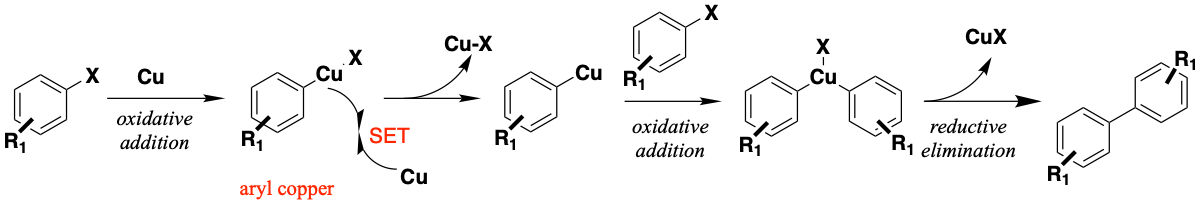
\includegraphics[width=1.0\columnwidth]{Fig/ullmann_mechanism.png}
%\caption{Mechanism of the Ullmann coupling reaction. SET stands for single-electron transfer.
%}
%\label{fig:classical}
%\end{figure}


%\textbf{Formation of organometallic intermediates on the Cu(111) surface.} Organic precursors are physisorbed on a metal surface before undergoing chemical transformations. Although the binding of chlorobenzene, bromobenzene and iodobenzene to Cu(111) calculated in this work is stronger than that obtained previously using the a different XC functional~\cite{jacs2013} the trends in the physisorption energies for different halogens are almost exactly the same (Table~\ref{table:bondlength}).

\begin{table*}
\centering
\caption{Characterization of the intermediates in the dehalogenation step on Cu(111). The energies are relative to \textbf{SURF}.
}
\label{table:bondlength}
\begin{tabular}{ llccccc  }
 \hline
 \hline
  & & & & Barrier & & Change \\
  & Hal. & \textbf{PHYS}$^{a}$ & \textbf{DHAL$\ddagger$}$^{b}$ & $\Delta^{(b-a)}$ & \textbf{DHAL}$^{c}$ & $\Delta^{(c-a)}$ \\ 
 \hline 
 \multirow{3}{*}{C--Hal (\si{\angstrom})} & Cl & 1.74 & 2.18 & +0.44 & 3.99 & +2.25 \\ 
 %\cline{2-5}
 & Br & 1.91 & 2.46 & +0.55 & 4.10 &+2.19 \\ 
 %\cline{2-5}
 & I & 2.12 & 2.61 & +0.49 & 5.10 &+2.98 \\ 
 %\cline{2-5}
 \hline
 \multirow{3}{*}{C--Cu (\si{\angstrom}) } & Cl & 3.54 & 2.52 & -1.02 & 2.01 & -1.53 \\ 
 & Br & 3.40 & 2.77 & -0.63 & 2.01 & -1.39 \\ 
 & I &3.42 & 2.73 &-0.69 & 2.01 & -1.41 \\ 
 \hline
 \multirow{3}{*}{Hal--Cu (\si{\angstrom}) } & Cl & 2.99 & 2.37 & -0.62 & 3.50 & +0.51 \\ 
 & Br & 2.89 & 2.50 & -0.49 & 3.57 & +0.68 \\ 
 & I &2.80 & 2.64 &-0.16 & 3.74 & +0.94 \\ 
 \hline
 \multirow{3}{*}{E (\si{\electronvolt}) } & Cl & -1.07 & 0.17 & 1.24 &-1.65 & -0.58 \\ 
 & Br &-1.14 &-0.25 & 0.89 & -1.95& -0.81 \\ 
 & I  & -1.32 & -0.69 & 0.63 & -2.28& -0.96 \\ 
 \hline
 \multirow{2}{*}{E (\si{\electronvolt})~\cite{jacs2013}} & Br &-0.95 & & 0.66 & & -0.68 \\ 
 & I & -1.12 & & 0.40 & & -0.81 \\ 
 \hline
 \hline
\end{tabular}
\end{table*}

\begin{figure*}[hbt]
\centering
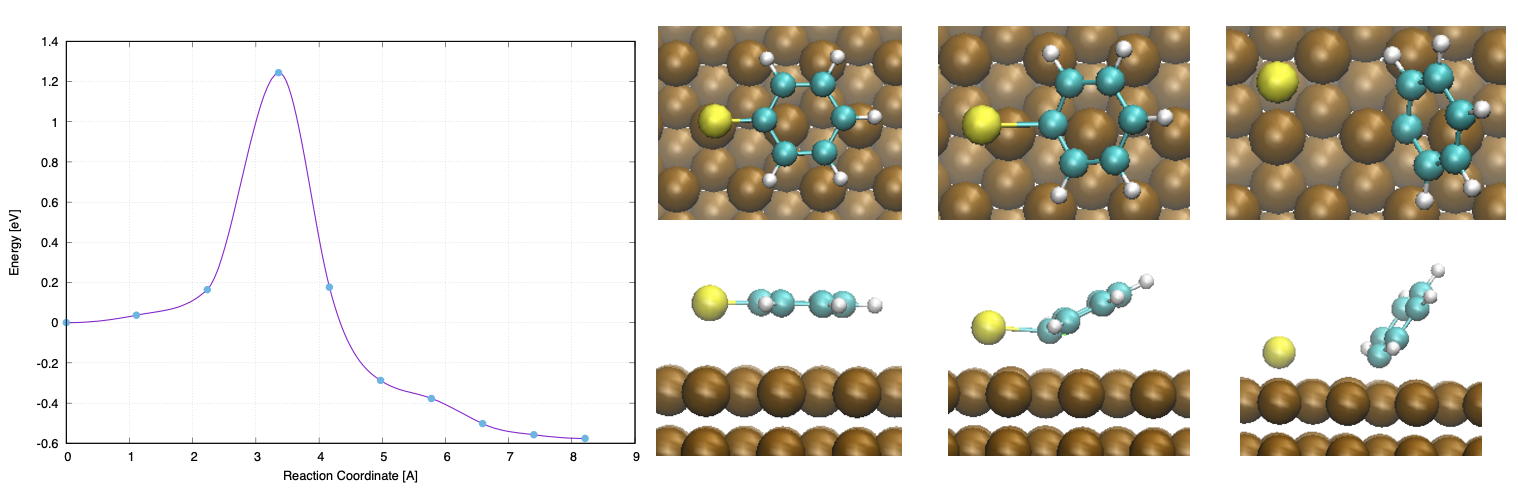
\includegraphics[width=1.0\textwidth]{Fig/dissociation_Cl.pdf}
\caption{Dissociation of the C--Cl bond on Cu(111). The energy diagram shows the NEB profile of the dechlorination process. In the structural images, orange, cyan, white, yellow spheres represent copper, carbon, hydrogen, chlorine atoms, respectively.}
\label{fig:dissociation_Cl}
\end{figure*}


\begin{figure*}[hbt]
\centering
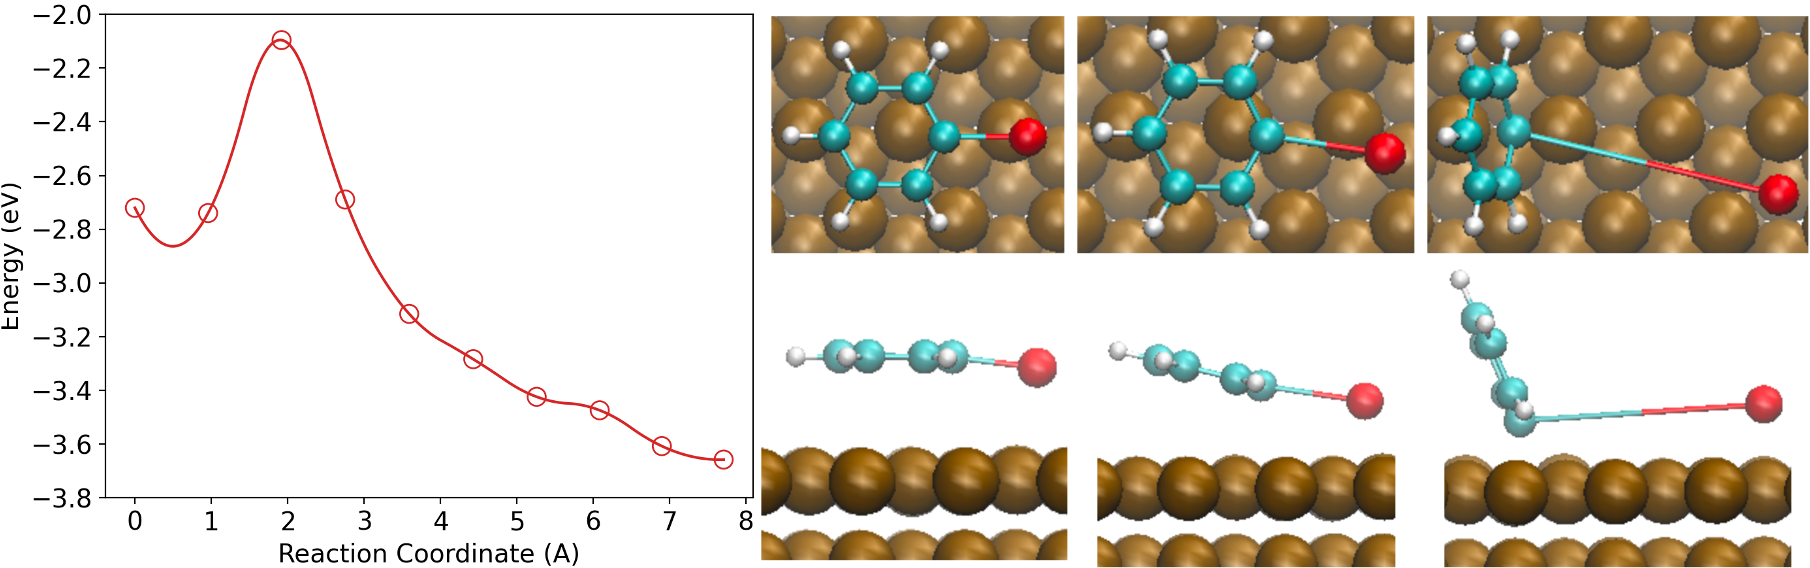
\includegraphics[width=1.0\textwidth]{Fig/dissociation_I.pdf}
\caption{Dissociation of the C--I bond on Cu(111). The energy diagram shows the NEB profile of the deiodination process. In the structural images, orange, cyan, white, purple spheres represent copper, carbon, hydrogen, iodine atoms, respectively.}
\label{fig:dissociation_I}
\end{figure*}

\begin{table*}
\centering\caption{Minimum experemental temperatures (\si{\kelvin}) necessary for the completion of the two key Ullmann compling steps.}
\begin{tabular}{ lcccccc }
 \hline
 \hline
  & \multicolumn{3}{c}{Dehalogenation} & \multicolumn{3}{c}{C--C bond formation} \\
  &\multicolumn{1}{c}{Cu} &\multicolumn{1}{c}{Ag} & \multicolumn{1}{c}{Au} & \multicolumn{1}{c}{Cu} &\multicolumn{1}{c}{Ag} &\multicolumn{1}{c}{Au}\\
 \hline
 Iodobenzene             &175\cite{sur_sci01} &200\cite{sur_sci02} &200-250\cite{sur_sci03} &350\cite{ullmann_68} &300-370\cite{ullmann_68} &250\cite{sur_sci03}\\
 Bromobenzene  &160\cite{ullmann_67} &$\leq$ 197\cite{sur_sci02}  &  &350\cite{ullmann_67}  &$\leq$ 350\cite{sur_sci02}  & \\
 Dichlorobenzene &420\cite{ullmann_52} & & &470\cite{ullmann_52} & & \\
 Dibromobenzene &$\leq$ 300\cite{ullmann_52} & & &470\cite{ullmann_98}  & & \\
 Diiodobenzene &$\leq$ 300\cite{ullmann_52} & & &500 \cite{ullmann_88} & & \\
 \hline
 \hline
\end{tabular}
\label{table:experimental-temperatures}
\end{table*}

\begin{table*}
\centering
\caption{Characterization of the intermediates in the $[1\bar{1}0]$ adatom pathway on Cu(111). Energies are reported relative to the \textbf{SURF} state.}
\label{table:adatom-110}
\begin{tabular}{ lccccccccccccc  }
 \hline
 \hline
 & & & & Barrier & & Change & & Barrier & &Change&\\
 & Met./Hal. & \textbf{CMC}$^{a}$ & \textbf{X-CMC$\ddagger$}$^{b}$ & $\Delta^{(b-a)}$ & \textbf{X-CMC}$^{c}$ &$\Delta^{(c-a)}$ & \textbf{X-DIM$\ddagger$}$^{d}$ & $\Delta^{(d-c)}$ & \textbf{X-DIM-A}$^{e}$ &$\Delta^{(e-c)}$ & \textbf{X-DIM-B}  \\ 
 \hline 
 {C--C (\si{\angstrom})} & Cu/Any & {3.10} & {3.55} & {+0.45} & {3.89} &{+0.79} & {2.53} &{-1.36} & {1.50} &{-2.39}\\ 
 \hline
 {C--Cu (\si{\angstrom}) } & Cu/Any & {2.06} & {1.85} & {-0.21} & {1.96} &{-0.10} & {1.90} &{-0.06} & {2.14} &{+0.18} &{} \\ 
 \hline
 {Cu$_{\rm lift}$ (\si{\angstrom}) } & Cu/Any & {0.53} & {1.68} & {+1.16} & {2.02} &{+1.49} & {1.77} & {-0.25} & {1.76} &{-0.26} &{0.00}\\ 
 \hline
 \multirow{3}{*}{E (\si{\electronvolt}) } & Cu/Cl & -3.05 &-1.67 & +1.38 &-3.26 &-0.21 & -1.25 & +2.01& -3.42&-0.16&-3.29 \\ 
 & Cu/Br &-3.73 &-2.35 &+1.38 & -3.94 &-0.21 & -1.93 & +2.01 & -4.11 & -0.16&-3.97 \\ 
 & Cu/I  & -4.38 & -3.00 & +1.38 & -4.59 &-0.21 & -2.58& +2.01 & -4.76 & -0.16&-4.62\\ 
 \hline
 \hline
\end{tabular}
\end{table*}

%\begin{figure*}[h!]
%\centering
%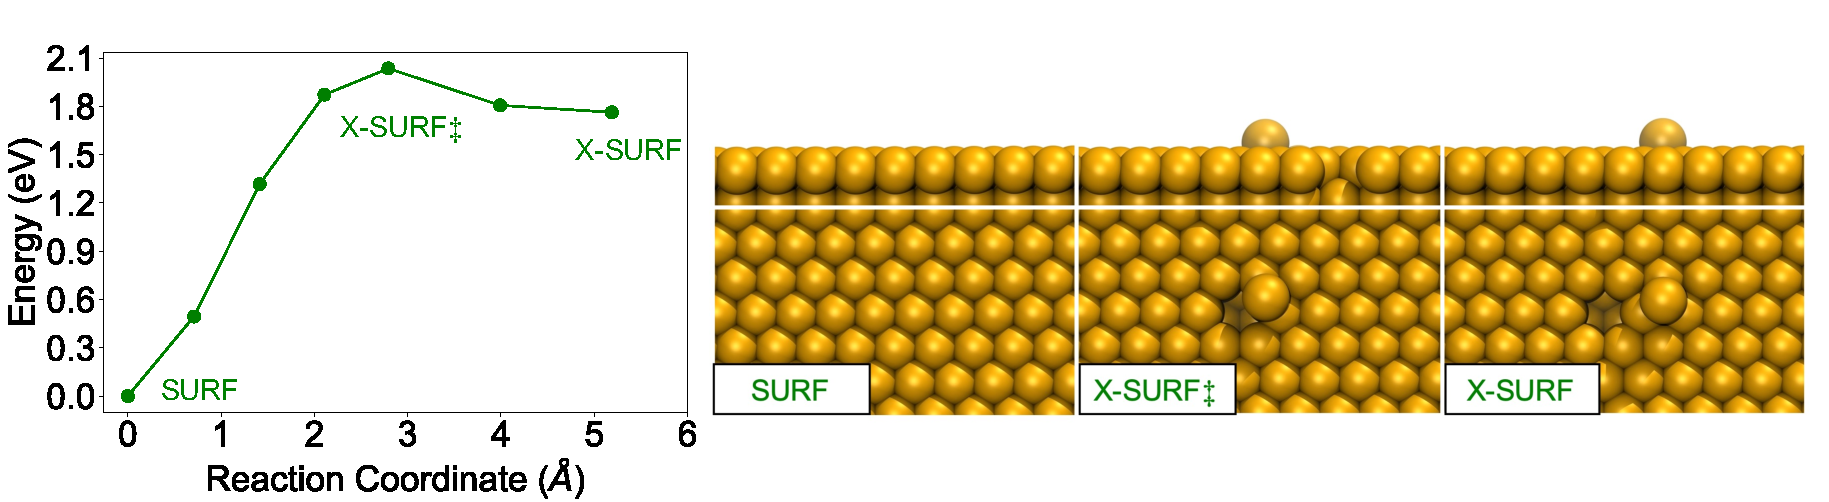
\includegraphics[width=1.0\textwidth]{Fig/pureadatomform.pdf}
%\caption{Energetics of an adatom formation on the clean Cu(111) surface.}
%\label{fig:cleanatomform}
%\end{figure*}

%\begin{figure}[hbt]
%\centering
%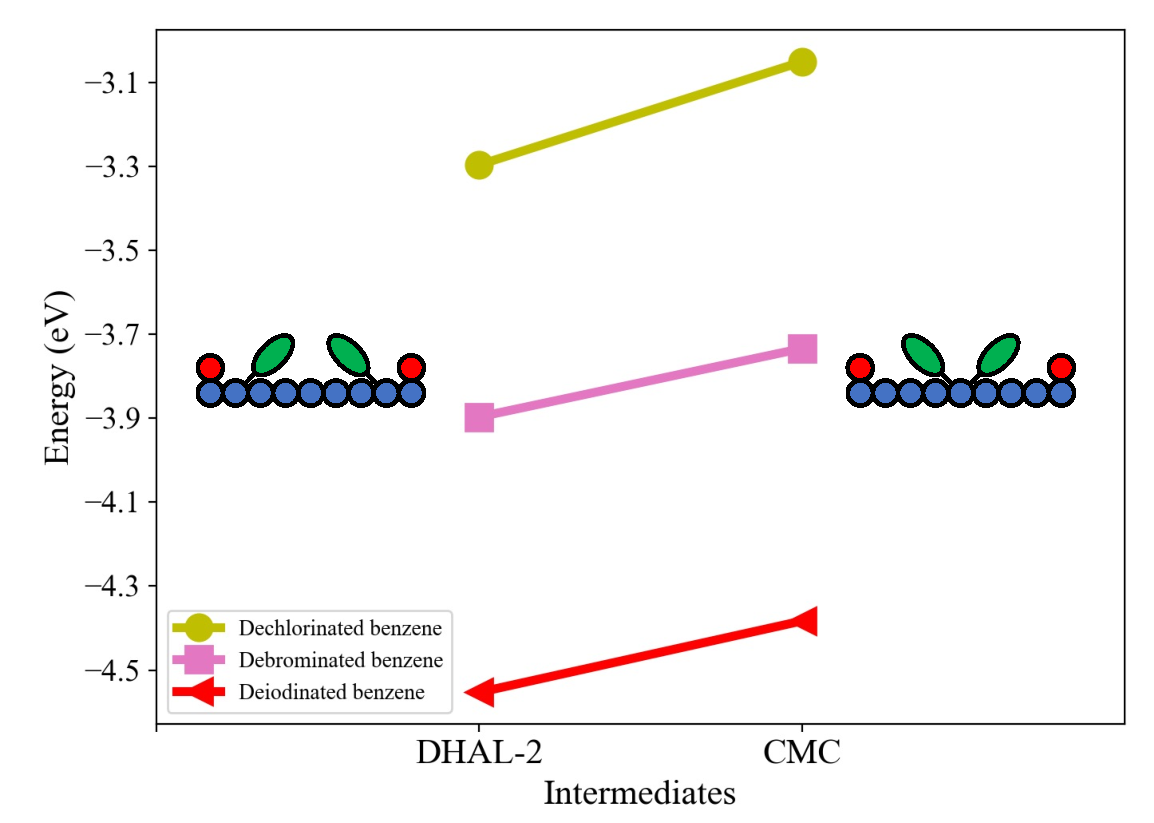
\includegraphics[width=0.45\textwidth]{Fig/FormingC-Cu-C.pdf}
%\caption{RZK0415: This figure is now obsolete and must be removed. It does not report any info complementary to the main energy profile.
%Energy diagram of forming C--Cu--C bridge intermediates structures from dechlorinated, debrominated and deiodinated benzene. The energy is computed as the difference between 2 $\times$ dehalogenated intermediates (left geometry) and C--Cu--C bridge intermediate structure $+$ two bromine atoms on Cu(111) surface. The blue circles represent chlorine, bromine or iodine atoms respectively in three situations. Yellow line with circle points is dechlorinated benzene to C--Cu--C, pink line with square points is debrominated benzene to C--Cu--C and red line with triangle points is deiodinated benzene to C--Cu--C.}
%\label{fig:formingBridge}
%\end{figure}

\section{Conditions for efficient adatom catalysis}

%The analysis of the three metals performed in this work raises a tantalizing question whether it is possible to find a metal surface capable of catalyzing the coupling of two phenyl groups through an efficient and competitive adatom pathway. 

The data collected in this work shows that the strengthening of the phenyl-adatom binding relative to the phenyl-surface binding -- further denoted as $X$ -- is important for two reasons. First, $X$ determines the energetics of the C--C bond formation step. For example, there is a nearly linear relation between $X$ and $\Delta B$ -- the difference in the C--C bond formation activation barriers in the adatom and ideal-surface pathways (Figure~\ref{main-fig:onlysurface}b):
% 
\begin{equation} \label{eq:relation1}
\Delta B = 0.9355 X
\end{equation}
%
Second, $X$ determines the energetics of the extraction step as well. As described in the main text, the energy required for the unassisted adatom extraction -- further denoted as $Y$ -- is compensated by $X$ when phenyl groups are bonded to the extracted adatom. It is reasonable to assume that metals with lower $Y$ (and the same $X$) will also have lower energy of phenyl-assisted extraction. For (hypothetical) metals with sufficiently low $Y$, the energetic cost of the adatom extraction will be fully compensated by $X$, resulting in the phenyl-assisted extraction that is thermoneutral.

To predict the energy of the phenyl-assisted extraction 

The line of thermoneutral extraction (TNE) is a shows what Y should a hypothetical metal with X have to exhibit the thermoneutral phenyl-assisted adatom extraction. Points lying below this line are characterized by exothermic assisted extraction and above this line by endothermic extraction. The vertical distance between a point $(X,Y)$ and the line is equal to the absolute energy of the phenyl-assisted adatom extraction:
%
\begin{equation}
\begin{split}
E_{\text{AEX}} = Y - \text{TNE}(X)
\end{split}
\end{equation}
%
where AEX - stands for assisted extraction.

The line of TNE is calculated by fitting a straight line to several points of TNE. Point of TNE is a point in the X-Y space at which the phenyl-assisted adatom extraction from the surface of a hypothetical metal is expected to have precisely zero energy.  The Y-position of a point of TNE is calculated from the DFT data for the metal by subtracting the energy of the phenyl-assisted adatom extraction from the clean-surface adatom extraction energy. The X-position of the point of TNE is assumed to be the same as the X-position of the metal described by DFT.



\bibliographystyle{achemso}
\bibliography{references}

\end{document}








